\documentclass[12pt,a4paper]{article}
% \usepackage[UTF8]{ctex}
% \usepackage{minted}
\usepackage{fontspec}
\usepackage{titletoc}
\usepackage{xeCJK}
\usepackage{graphicx}
\usepackage{amsmath}
\usepackage{indentfirst} % 中文首段缩进
\usepackage{minted} % 代码块高亮渲染

\setmainfont[Path=/usr/share/fonts/wenquanyi/wqy-microhei/]{wqy-microhei.ttc}
\setCJKmainfont[Path=/usr/share/fonts/wenquanyi/wqy-microhei/]{wqy-microhei.ttc}

\graphicspath{ {img/} }

\usepackage{xcolor}
\usepackage{hyperref}
\hypersetup{
    colorlinks=true,
    linkcolor=blue,
    urlcolor=red,
    linktoc=all
}
\definecolor{bg}{rgb}{0.95,0.95,0.95}
\newcommand{\incode}[1]{\mintinline[bgcolor=bg]{c}{#1}} % 定义行内代码渲染命令
\renewcommand{\baselinestretch}{1.1} % 定义行间距
\parindent 24pt % 重新定义缩进长度
 
%%%%%%%%%%%%%%%%%%%%%%%%%%%%%%%%%%%%%%%%%%%%%%%%%%%%%%%%%%%%%%%%
%  lengths
%    下面的命令重定义页面边距,使其符合中文刊物习惯。
%%%%%%%%%%%%%%%%%%%%%%%%%%%%%%%%%%%%%%%%%%%%%%%%%%%%%%%%%%%%%%%%
\addtolength{\topmargin}{-54pt}
\setlength{\oddsidemargin}{-0.9cm}  % 3.17cm - 1 inch
\setlength{\evensidemargin}{\oddsidemargin}
\setlength{\textwidth}{17.00cm}
\setlength{\textheight}{24.00cm}    % 24.62

\title{实验二~多周期MIPS~CPU}
\author{张海斌\thanks{学号 17307130118}}
\begin{document}
\date{2019年5月}

\maketitle

\renewcommand\contentsname{目~录}
\tableofcontents

\section{概要}

多周期处理器与单周器处理器相比有很多相似的地方,比如都可以分为控制器和数据通路两大部份,都需要除通用寄存器外的寄存器存储程序运行状态(如需要寄存器记录PC位置)。多周期处理器与单周器处理器中,有许多部件也是可以通用的。但是在存储器上有一点区别是多周期处理器中需要执行的机器代码与内存空间是在同一存储空间中,这也就更符合冯·诺依曼体系结构。

\section{功能展示}

LED[3:0]四位显示当前多周期处理器的状态的二进制编码,状态编码方式见Table \ref{table:state}。LED[15]显示CPU时钟信号状态。从左向右前两个七段数码管显示当前PC值,接着的两个数码管显示写入PC使能寄存器的值(只有当有使能信号的时候才会写入PC),最后四位七段数码管显示内存或寄存器中的值。
SW[0]控制状态的清零,SW[1]控制CPU的运行和暂停,SW[9:4]提供需要查看的寄存器或内存的地址:当SW[2]为0时,以SW[8:4]的内容为寄存器地址,显示相应寄存器中的数据在右侧四个七段数码管上;当SW[2]为1时,以SW[9:4]的内容为内存地址,在相同的七段数码管上显示内存的数据。

\begin{table}
	\centering
	\begin{tabular}{|c|c|c|}
		\hline
		状态名称 & 状态编码 & 解释\\
		\hline
		FETCH    &  4'b0000 & 取指令\\
		DECODE   &  4'b0001 & 解码机器指令\\
		MEMADR   &  4'b0010 & \incode{lw}或\incode{sw}指令中计算内存地址\\
		MEMRD    &  4'b0011 & 读取内存数据\\
		MEMWB    &  4'b0100 & 写回数据到寄存器中\\
		MEMWR    &  4'b0101 & 写回数据到内存中\\
		REX      &  4'b0110 & R-Type指令执行阶段(进行计算)\\
		RWB      &  4'b0111 & R-Type指令计算结果写回寄存器\\
		BEX      &  4'b1000 & \incode{beq}或\incode{bne}指令执行阶段\\
		IEX      &  4'b1001 & I-Type指令执行阶段\\
		IWB      &  4'b1010 & I-Type指令写回阶段\\
		JEX      &  4'b1011 & \incode{jump}指令执行阶段\\
		\hline
	\end{tabular}
	\caption{有限状态机状态编码}
	\label{table:state}
\end{table}

\section{代码结构}

\begin{figure}[h]
	\centering
	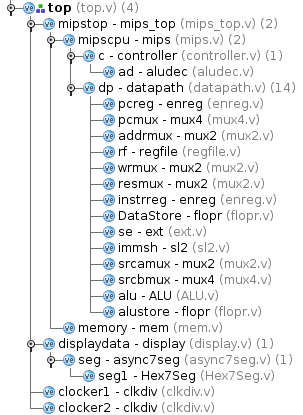
\includegraphics[width=0.5\textwidth]{struct}
	\caption{Verilog模块层次结构图}
	\label{fig:struct}
\end{figure}

Figure \ref{fig:struct} 展现了Verilog中各个模块的层次结构。\incode{top}是上板子的顶层文件,下面有两大模块\incode{mips_top}\ \incode{display}及两个时钟分频器 \incode{clkdiv}。\incode{mips_top}和\incode{display},分别为多周期处理器的顶层模块和负责处理板子显示的模块。在显示模块中包括了处理八个七段数码管连续显示的\incode{async7seg}模块,而它下含的\incode{Hex7Seg}则是将十六进制数转化为七段数码管上数字或字母显示的信号。\incode{mips_top}模块下主要分为两个模块:\incode{controller}控制器和\incode{datapath}数据通路。

\section{模块设计}

\incode{display}模块中,主要是使用\incode{case}语句判断信号条件,从而决定七段数码管右侧四个所要展示的数据(见Listing \ref{code:display}),另一方面为了避免暂停CPU的时候导致时钟暂停,从而影响不同的七段数码管同时显示数据的功能,我在\incode{top}模块中使用了两个时钟分频模块\incode{clkdiv}分别为CPU和七段数码管的显示提供时钟信号。

\begin{listing}[ht]
	\definecolor{bg}{rgb}{0.95,0.95,0.95}
	\begin{minted}[bgcolor=bg,linenos]{verilog}
        case(Ctl[0])
            1'b0:
            begin
                DispReadReg <= Addr[4:0];
                DispReadMem <= 6'b0;
                Data[15:0] <= DispRegData;
            end
            1'b1:
            begin
                DispReadReg <= 5'b0;
                DispReadMem <= Addr;
                Data[15:0] <= DispMemData[15:0];
            end
        endcase
	\end{minted}
	\caption{\incode{display}模块数据显示的选择}
	\label{code:display}
\end{listing}

在多周期处理器中,由于保存PC的寄存器受到使能信号的控制,需要设计新的带使能端的寄存器\incode{enreg}。还有在数据通路中,出现了四选一多路选择器,这也需要添加相应模块。而其它的一些基本模块不需要进行修改,其中包括接收是否需要符号位扩展信号的扩位器\incode{ext}、时钟沿触发器\incode{flopr}、运算单元\incode{ALU}、左移两位的移位器\incode{sl2}、二选一多路选择器\incode{mux2}和寄存器文件\incode{regfile}。内存模块中新添加了初始化代码,这原本是在指令内存\incode{imem}中进行的操作,而现在在我们的多周期处理器中内存同时肩负保存运行的机器指令以及内存数据的职责,具体代码可以参考Listing \ref{code:mem}。

\begin{listing}[ht]
    \begin{minted}[bgcolor=bg,linenos]{verilog}
module mem(
    input CLK, WE,
    input [31:0] A, WD,
    output [31:0] RD,
    input [5:0] ReadAddr,
    output [31:0] Data);
// Instruction and Data Memory
    reg [31:0] RAM[63:0];

    initial
        $readmemh("/PAHT/TO/memfile.dat", RAM); // $
    assign RD = RAM[A[31:2]];
    assign Data = RAM[ReadAddr];

    always @(posedge CLK)
        if (WE)
            RAM[A[31:2]] <= WD;
        else
            RAM[A[31:2]] <= RAM[A[31:2]];
endmodule
	\end{minted}
	\caption{\incode{mem}内存模块}
	\label{code:mem}
\end{listing}

在CPU顶层文件\incode{mips_top}中包括\incode{mips}CPU核心模块和数据存储的内存模块\incode{mem},以及在\incode{mips}CPU核心模块中包括控制器\incode{controller}和数据通路\incode{datapath}都不需要进行过多的解释说明。

\section{数据通路}

\begin{figure}[h]
	\centering
	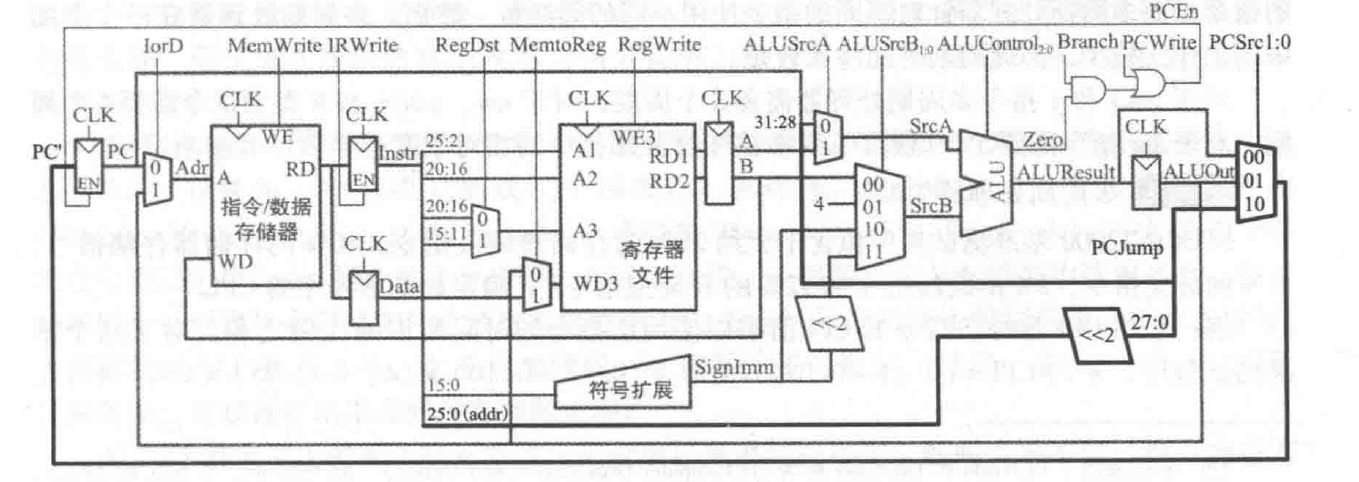
\includegraphics[width=\textwidth]{datapath}
	\caption{多周期数据通路线路图}
	\label{fig:datapath}
\end{figure}

数据通路模块\incode{datapath}这一部份我大部份是按照Figure \ref{fig:datapath}中的线路进行连接,不过有几个地方我进行了修改。一个是寄存器文件输出\incode{RD1}和\incode{RD2}后有一个寄存器,它被用来稳定\incode{A}和\incode{B}的信号。因为在一条指令周期中没有非常必要的作用我将它删去了。由于在I-Type指令中存在位操作运算,所以需要对16位的立即数进行0扩展,因此数据通路中的扩位器需要有有符号和无符号扩展两种操作,同时需要一位信号\incode{ExtOp}来控制这个模块的操作。最后一点不同在于,书中\incode{PCEn}是在数据通路中通过\incode{Zero}、\incode{Branch}和\incode{PCWrite}三个信号的逻辑操作得到的,而我将\incode{PCEn}信号的生成放在了控制器\incode{controller}中。也就是说,数据通路将\incode{Zero}信号传递给\incode{controller},然后\incode{controller}将\incode{PCEn}信号回传给数据通路。

数据通路中,我认为值得注意的一个地方是内存与寄存器文件之间的\incode{Data}寄存器与\incode{ALUResult}与\incode{ALUOut}之间的寄存器。它们的存在让进入的数据信号晚一个时钟周期才向后传递。这在控制信号的设计中需要注意理解。

\section{控制器}

多周期处理器中控制器信号要比单周器控制器更加复杂,因为多周期处理器中一条指令需要多个时钟周期才嫩完成,在执行同一条指令中的不同时钟周期中,控制信号也会有所差异,而单周器处理器在每个周期内只需要根据机器指令生成对应的控制信号。我使用了有限状态机来实现这个控制器。Table \ref{table:state}列出了有限状态机的状态编码。不过其中I-Type我并不是指所有的I-Type指令,而是代表I-Type中所有类似于R-Type指令使用ALU进行数据计算并将结果写回到寄存器中的运算指令。

所以在控制器中,我将多种I-Type指令的状态合并到一起,用\incode{IEX}和\incode{IWB}代表它们的状态。而当前状态用四位的寄存器\incode{state}储存。

\begin{figure}[h]
	\centering
	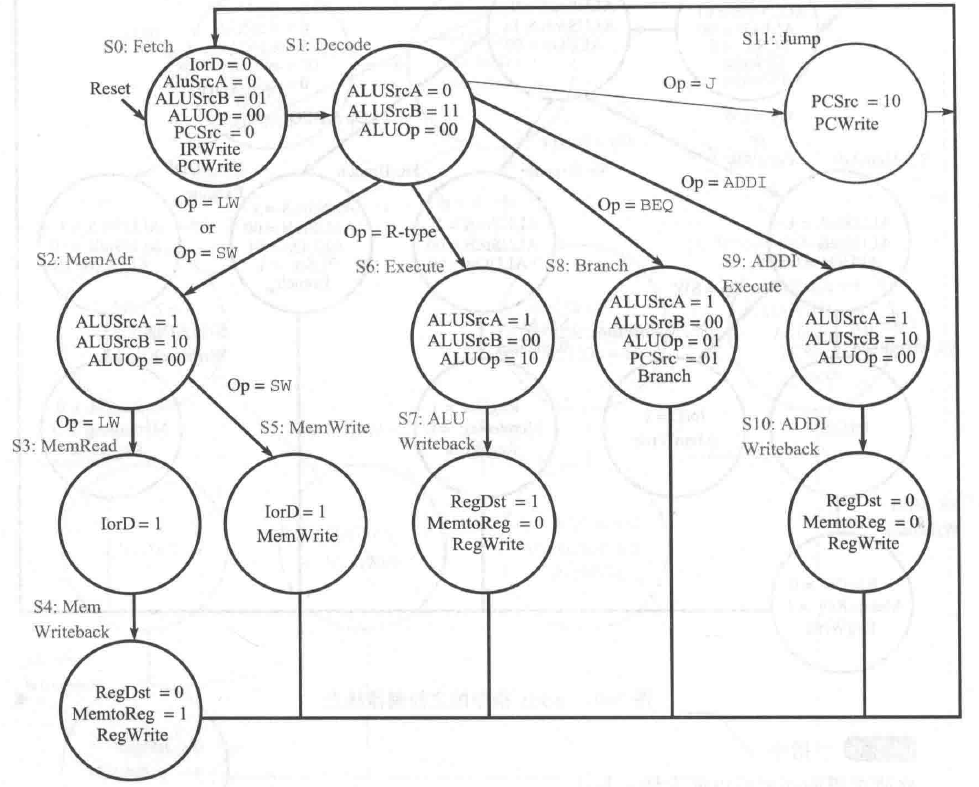
\includegraphics[width=\textwidth]{state}
	\caption{控制器状态转移图}
	\label{fig:state}
\end{figure}

在状态转移图中,我将\incode{beq}和\incode{bne}的状态合并在一起,将多个I-Type的状态合并到一起,减少了状态的总数,但同时输出信号的逻辑运算过程更加复杂了。\incode{beq}和\incode{bne}的六位操作码中,只有最低位不同,因此我用\incode{assign bne = Op[0];}获得是否为\incode{bne}的信号,然后由\incode{assign PCEn = ((Zero ^ bne) & Branch) | PCWrite;}得到\incode{PCEn}的结果。\incode{Branch}只有在处于状态\incode{BEX}的时候才是1;在状态不是\incode{BEX}的时候,\incode{Branch}始终为0,所以此时\incode{PCEn}只受到\incode{PCWrite}的控制,不会造成异常。代码见Listing \ref{code:branch}。

\begin{listing}[ht]
    \begin{minted}[bgcolor=bg,linenos]{verilog}
    // Branch 只有在 BEQ 或 BNE 的执行阶段才为 1
    always @(*)
        if (state == BEX)
            Branch <= 1;
        else
            Branch <= 0;
	\end{minted}
	\caption{\incode{Branch}信号控制}
	\label{code:branch}
\end{listing}

对于\incode{ALUCtl}ALU控制信号的产生上,我会从两个\incode{ALUOp}中选择一个传递到\incode{ALUCtl}。其中,\incode{ALUOp0}是根据有限状态机当前状态生成的,而\incode{ALUOp1}是只根据Op Code和Funct而决定的在执行阶段所需要的ALU控制信号,它是由模块\incode{aludec}生成的,随之一起生成的信号还与\incode{ExtOp1}扩位运算信号。当处于\incode{REX}或\incode{IEX}状态时,会使用\incode{ALUOp1}信号与\incode{ExtOp1}信号作为输出信号,其它情况都会使用\incode{ALUOp0}信号与\incode{ExtOp0}信号作为输出。另外,\incode{ExtOp1}信号始终为1。相关代码见Listing \ref{code:muxalu}。

\begin{listing}[ht]
    \begin{minted}[bgcolor=bg,linenos]{verilog}
    // AluCtl 和 ExtOp 的在 R-Type/I-Type Execute 阶段的特殊控制
    always @(*)
        if (state == REX || state == IEX)
            {AluCtl, ExtOp} <= {AluOp1, ExtOp1};
        else
            {AluCtl, ExtOp} <= {AluOp0, ExtOp0};
	\end{minted}
	\caption{\incode{ALUOp}和\incode{ExtOp}信号控制}
	\label{code:muxalu}
\end{listing}

所以\incode{aludec}模块的作用就是根据Op Code和Funct生成在执行阶段所需要的\incode{ALUOp}和\incode{ExtOp}信号。这两个信号也只有在\incode{REX}或\incode{IEX}状态时才会被使用。通过这种方法避免了不同的I-Type需要添加不同的状态。

在\incode{controller}模块中,分别有一个\incode{case}语句来判断有限状态机的下一个周期的状态以及生成当前状态下的输出信号,这部份输出信号被并为了总线\incode{ctls}。\incode{assign {PCWrite, MemWrite, IRWrite, RegWrite, ALUSrcA, IorD, MemToReg, RegDst, ALUSrcB, PCSrc, AluOp0} = ctls;}这是\incode{ctls}的连线情况。而下一周期的状态由当前状态和Op Code共同决定。

\section{多周期状态转移的改进}

在列出了状态输出表之后,我发现在某些状态下使用的部件非常少,有的不同周期可以进行合并。\incode{MEMWB}、\incode{RWB}、\incode{IWB}三个状态与\incode{FETCH}状态的有效输出信号恰好相错开,也就是说,我们可以在前三个状态执行的同时,将下一个指令周期的\incode{FETCH}阶段的工作同时完成掉。这样,执行完前三个状态后,可以直接跳到\incode{DECODE}阶段。而这对程序的运行没有任何影响。而且这个改进过程只涉及到了相关状态的状态转移和状态输出的改变,比较容易实现。

修改前后,仿真跑出来的时间分别为620ns和510ns,说明这个优化对处理器运行速度的提升还是比较明显的。

\section{仿真结果}

\begin{figure}[h]
	\centering
	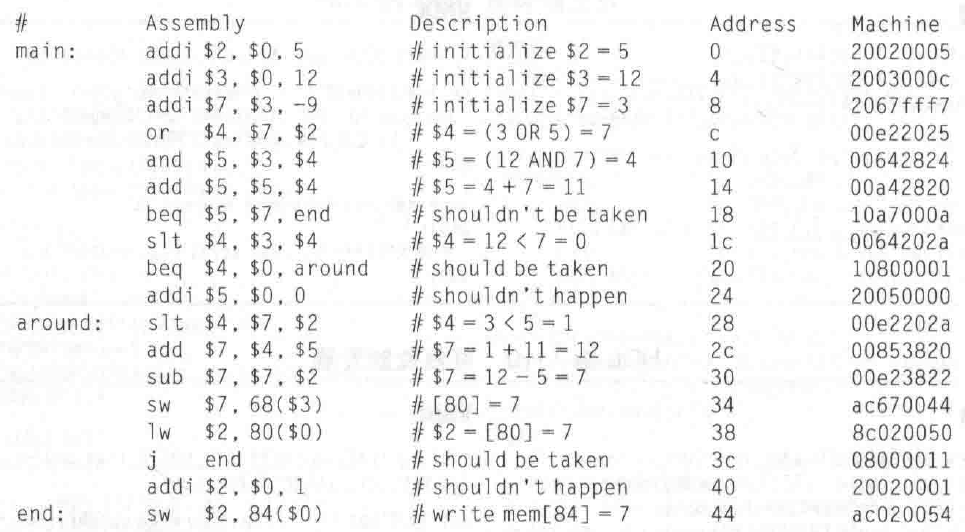
\includegraphics[width=\textwidth]{code}
	\caption{测试代码}
	\label{fig:code}
\end{figure}

Figure \ref{fig:code}是测试用的代码。Figure \ref{fig:seq1-1}和Figure \ref{fig:seq1-2}是没有优化状态转移前的代码测试结果;Figure \ref{fig:seq2-1}和Figure \ref{fig:seq2-2}是优化状态转移后的代码测试结果。其中需要注意的地方是,\incode{PC}并不一定代表当前执行代码的位置,因为在\incode{FETCH}阶段会将\incode{PC}加4并写入\incode{PC},这样\incode{PC}就指向下一条指令了,但实际上处理器还没有执行到下一条指令。同理,对于跳转指令\incode{jump}或\incode{beq}或\incode{bne},只有根据下一个状态为0的时候的\incode{PC}的值才能判断是否发生了跳转。

\begin{figure}[h]
	\centering
	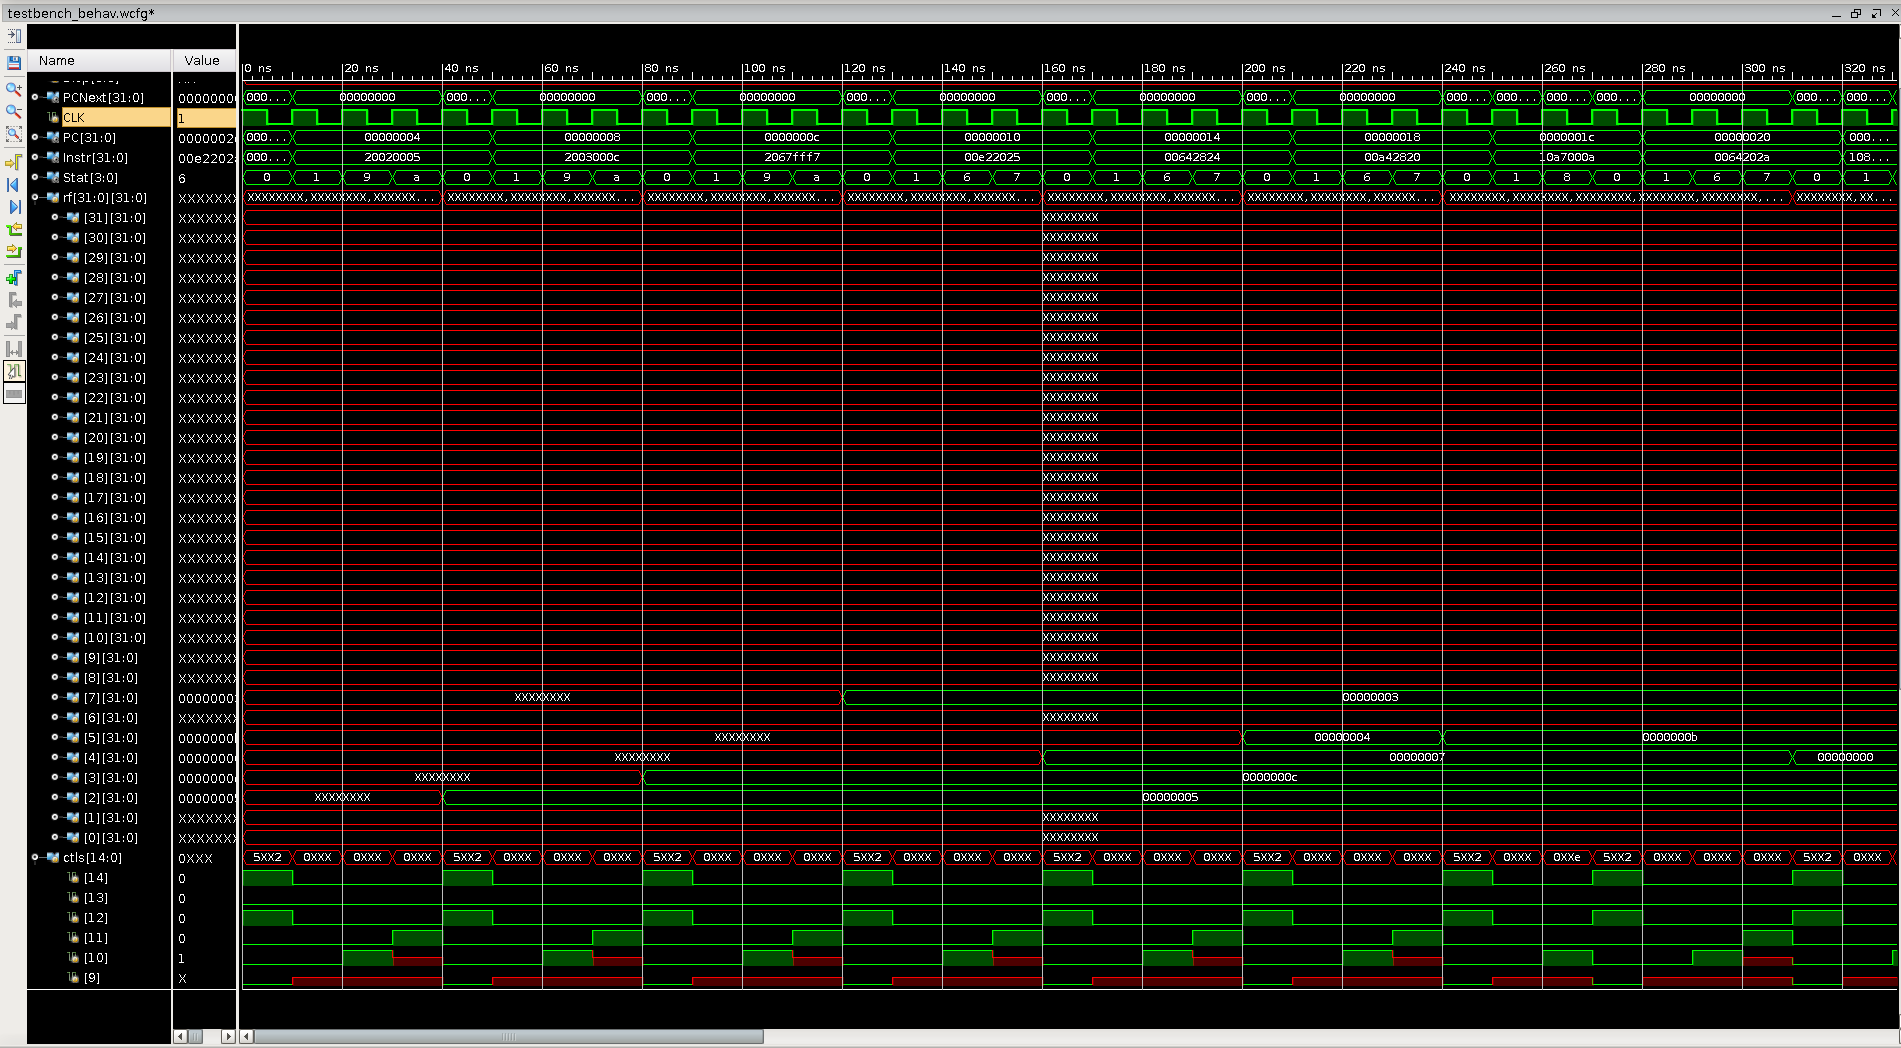
\includegraphics[width=\textwidth]{seq1}
	\caption{状态转移未优化~左图}
	\label{fig:seq1-1}
\end{figure}

\begin{figure}[h]
	\centering
	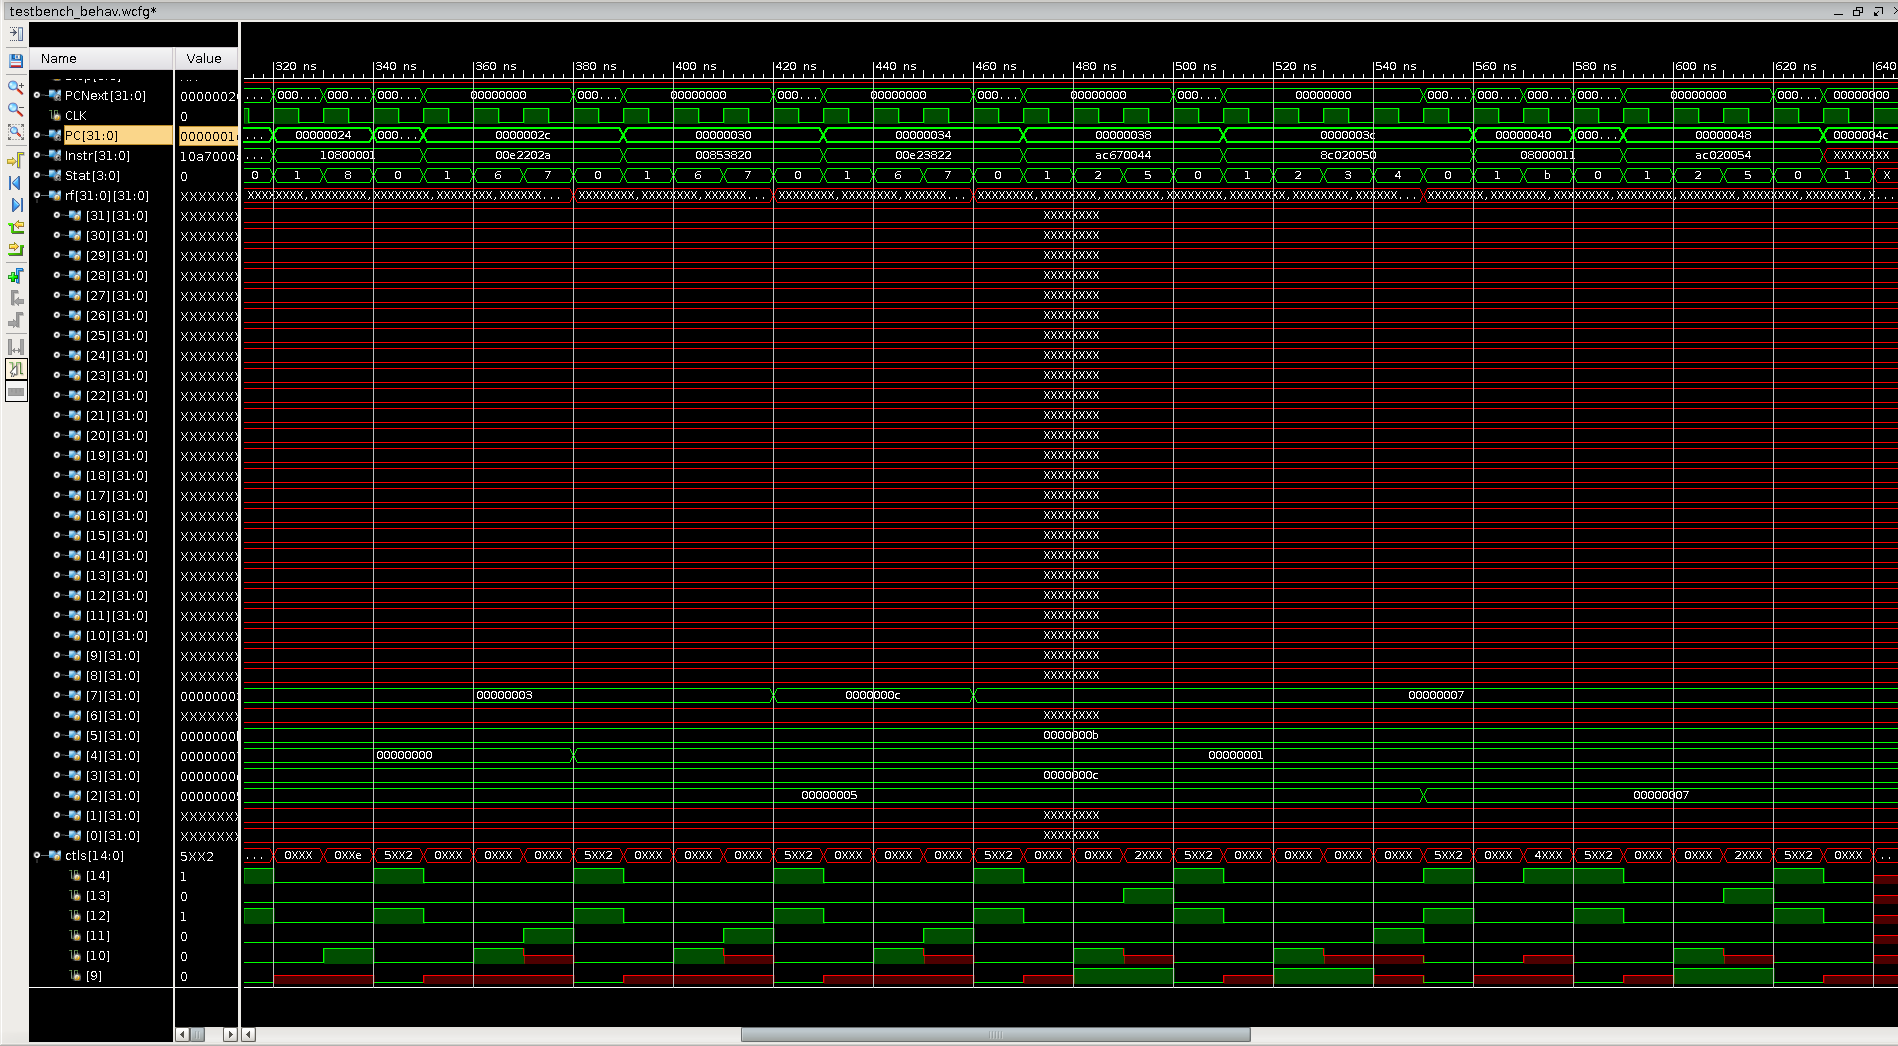
\includegraphics[width=\textwidth]{seq2}
	\caption{状态转移未优化~右图}
	\label{fig:seq1-2}
\end{figure}

\begin{figure}[h]
	\centering
	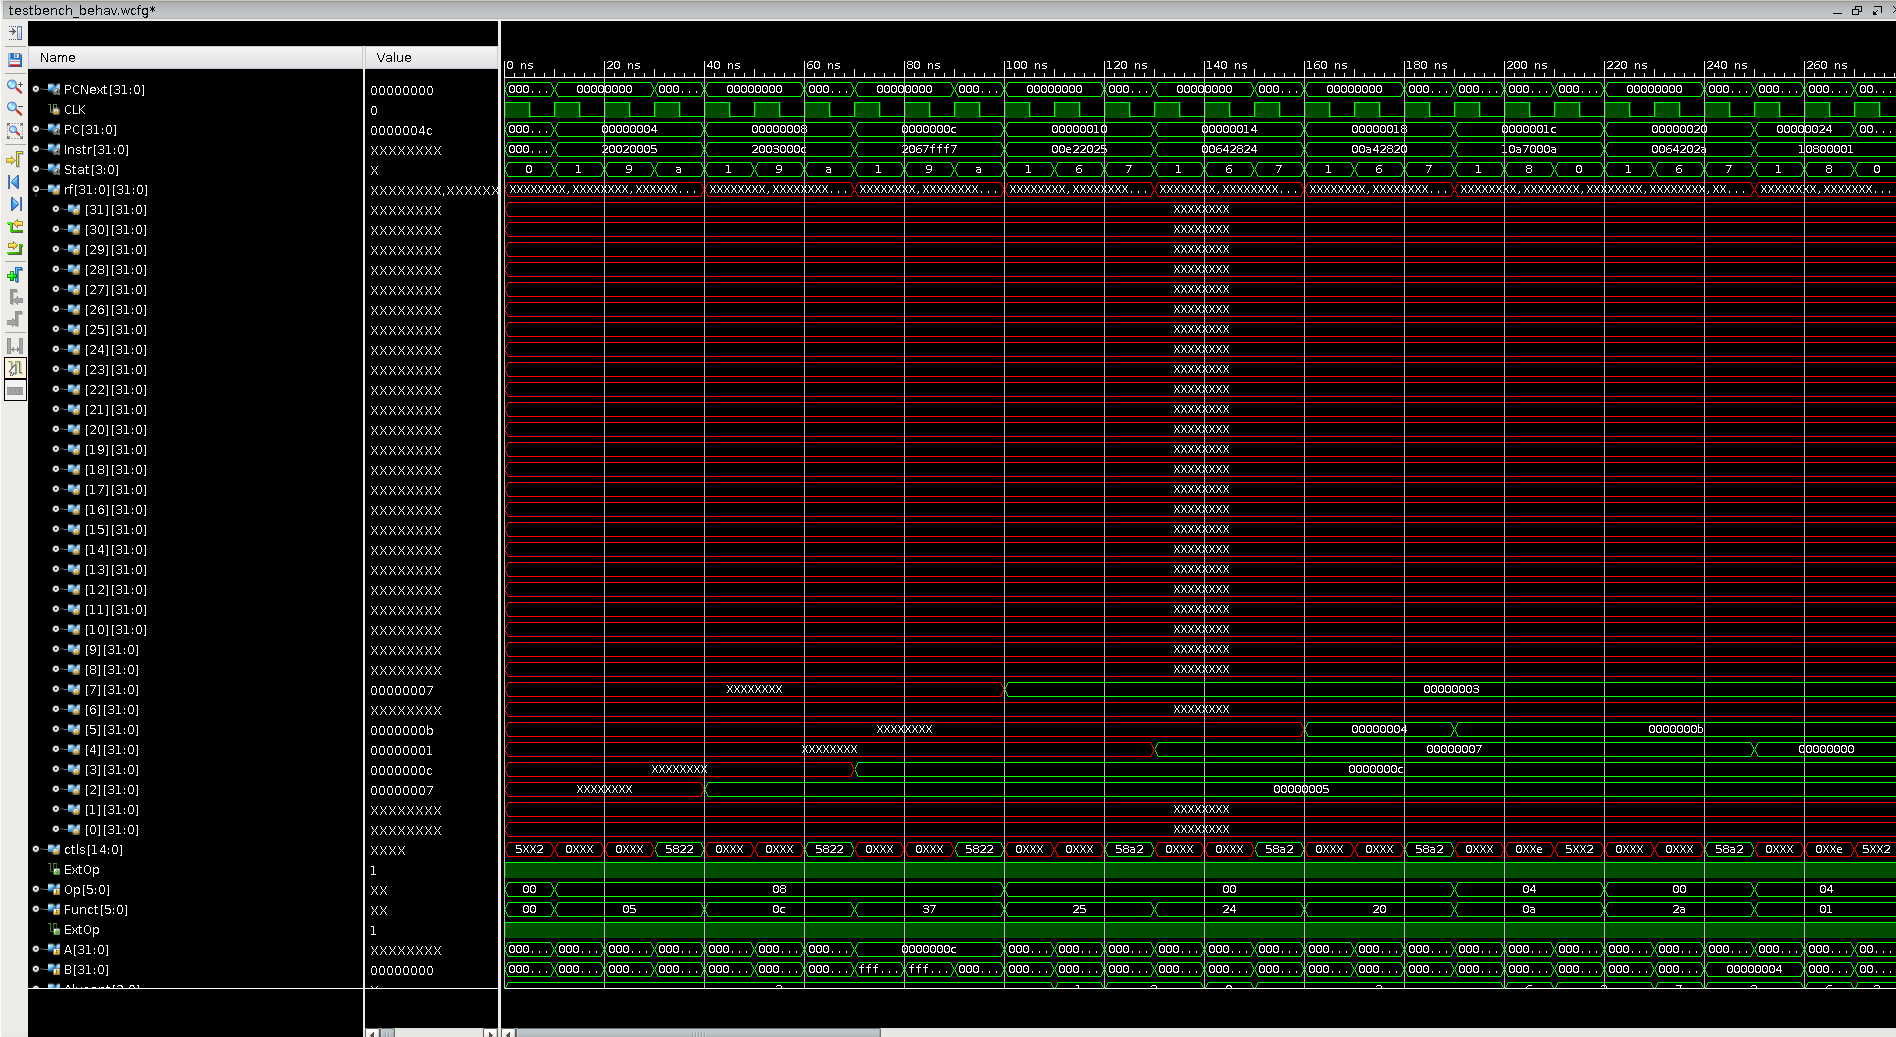
\includegraphics[width=\textwidth]{seq3}
	\caption{状态转移已优化~左图}
	\label{fig:seq2-1}
\end{figure}

\begin{figure}[h]
	\centering
	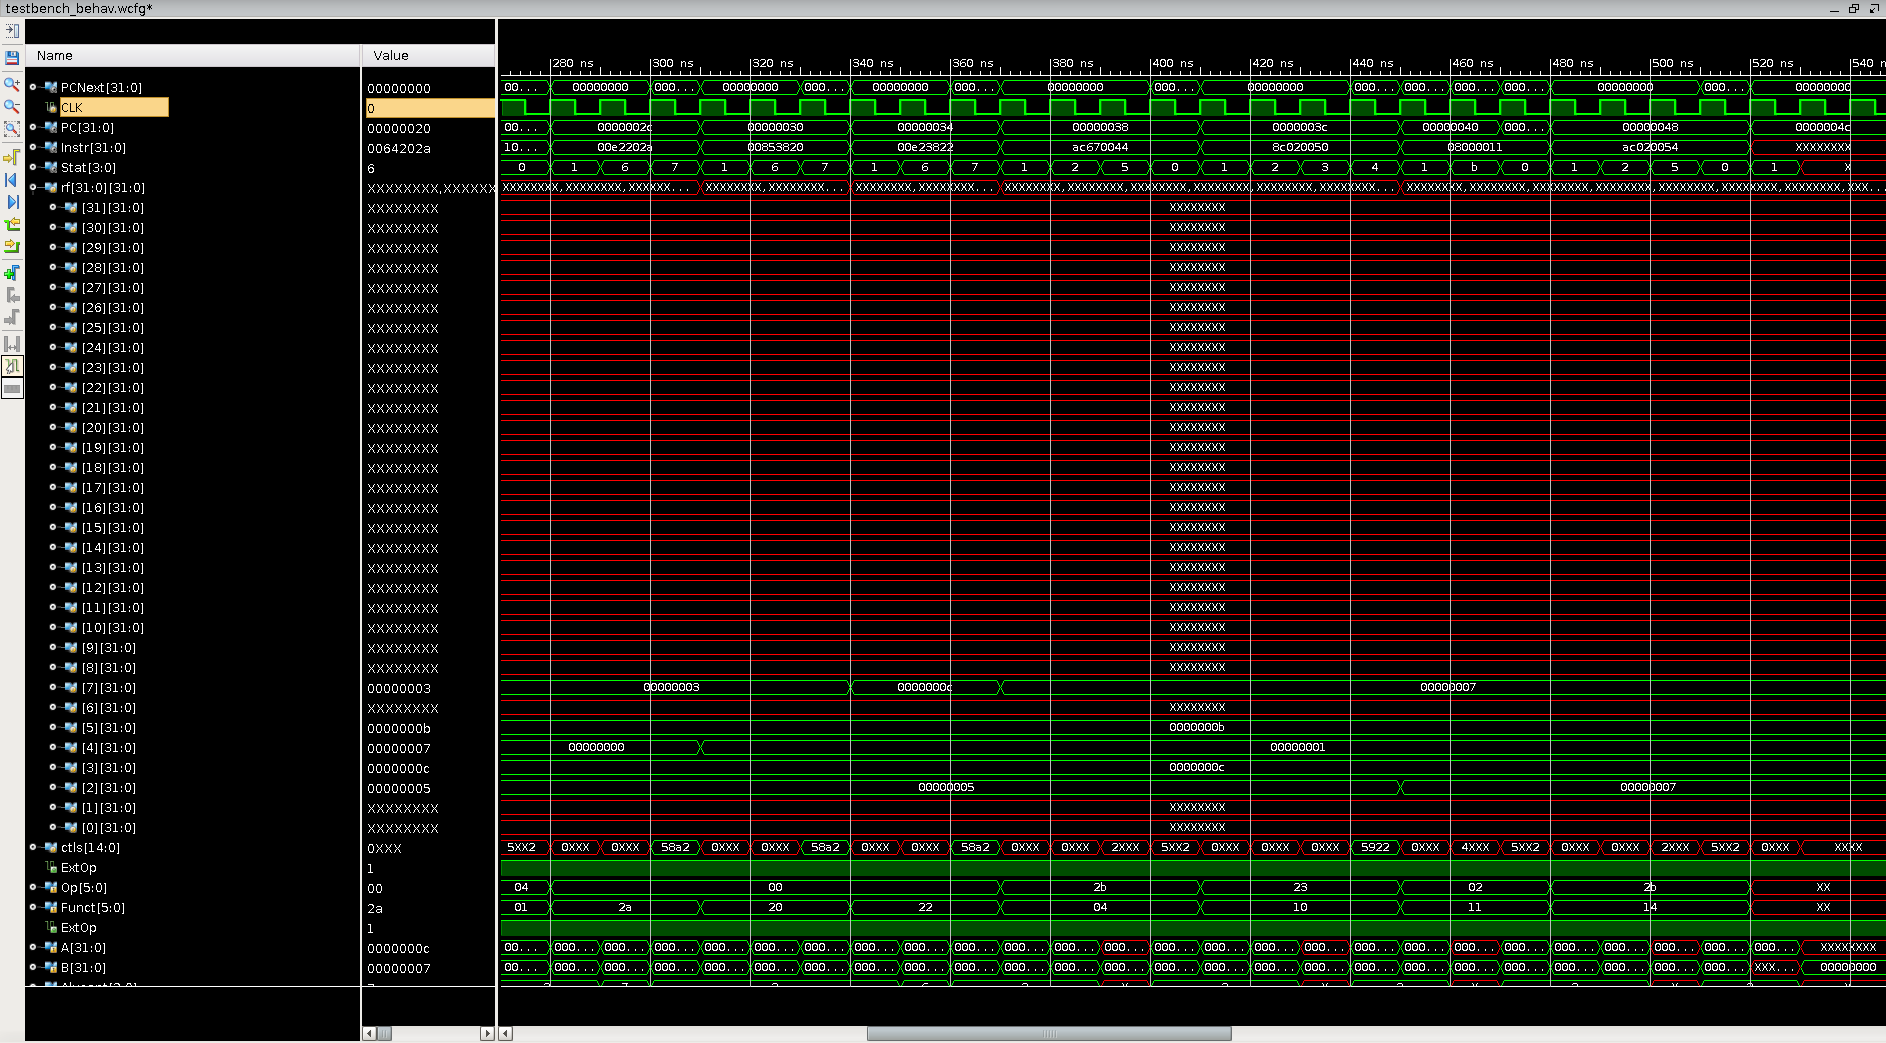
\includegraphics[width=\textwidth]{seq4}
	\caption{状态转移已优化~右图}
	\label{fig:seq2-2}
\end{figure}
\end{document}
